% THIS IS SIGPROC-SP.TEX - VERSION 3.1
% WORKS WITH V3.2SP OF ACM_PROC_ARTICLE-SP.CLS
% APRIL 2009
%
% It is an example file showing how to use the 'acm_proc_article-sp.cls' V3.2SP
% LaTeX2e document class file for Conference Proceedings submissions.
% ----------------------------------------------------------------------------------------------------------------
% This .tex file (and associated .cls V3.2SP) *DOES NOT* produce:
%       1) The Permission Statement
%       2) The Conference (location) Info information
%       3) The Copyright Line with ACM data
%       4) Page numbering
% ---------------------------------------------------------------------------------------------------------------
% It is an example which *does* use the .bib file (from which the .bbl file
% is produced).
% REMEMBER HOWEVER: After having produced the .bbl file,
% and prior to final submission,
% you need to 'insert'  your .bbl file into your source .tex file so as to provide
% ONE 'self-contained' source file.
%
% Questions regarding SIGS should be sent to
% Adrienne Griscti ---> griscti@acm.org
%
% Questions/suggestions regarding the guidelines, .tex and .cls files, etc. to
% Gerald Murray ---> murray@hq.acm.org
%
% For tracking purposes - this is V3.1SP - APRIL 2009

\documentclass{acm_proc_article-sp}

%% Additional packages
\usepackage{amsmath}
%\usepackage{amsthm}
\usepackage{amssymb}
\usepackage{amsfonts}
%\usepackage{mathtools}
%\usepackage{calc}
%\usepackage{subfigure}
\usepackage{graphicx}
\usepackage{color}
\usepackage{url}
%\usepackage{lineno}
%\usepackage{ulem} % for underlining and strike through
%\normalem % reset emph to normal
%\usepackage{setspace} % for line spacing - e.g. 1.5, 2
\usepackage[usenames,dvipsnames]{xcolor}
\usepackage{xspace} % for inserting a space in TeX commands if needed
\usepackage{caption}
\usepackage{hyperref}
%\renewcommand{\thesubfigure}{\relax} % no subfig counters
%\let\chapter\section % algorithm2e natbib compatibility
%\usepackage{accents}

%% Packages
%\usepackage[margin=1in]{geometry}
%\usepackage[abs]{overpic}
\usepackage[linesnumbered,vlined,ruled]{algorithm2e}
%\usepackage{multirow} % for cell tables spanning multiple rows
%\usepackage{tikz,pgf}%,tikz-3dplot}
%\usetikzlibrary{arrows,automata,shapes,calc,backgrounds,spy}
%\usetikzlibrary{external}
%\tikzexternalize
%\usepackage[sort,round]{natbib}
%\usepackage{lipsum}
\usepackage{verbatim}

%\usepackage[author={Cristi}]{pdfcomment}

%%% figure path
\graphicspath{{figures/}}

%% Remove footnote mark
%\renewcommand{\footnotemark}{}

%%% Redefine qed symbol
%\renewcommand{\qedsymbol}{$\blacksquare$}

%% Projection symbol
%\newcommand{\project}[1]{\! \upharpoonright_{#1}}


%% Theorems
\newtheorem{theorem}{Theorem}[section]
\newtheorem{proposition}[theorem]{Proposition}
\newtheorem{corollary}[theorem]{Corollary}
\newtheorem{definition}{Definition}[section]
\newtheorem{lemma}[theorem]{Lemma}
\newtheorem{remark}[theorem]{Remark}
\newtheorem{remarks}[theorem]{Remarks}
\newtheorem{example}{Example}[section]
\newtheorem{algo}{Algorithm}
\newtheorem{problem}{Problem}[section]
\newtheorem{Procedure}[theorem]{Procedure}
\newtheorem{assumption}{Assumption}
%\newcommand{\exampler}[2]{\medskip \hskip -\parindent {\bf Example #1 Revisited.~}{\it #2}\medskip}

%% Percent
%\newcommand\oprocendsymbol{\hbox{$\square$}}
%\newcommand\oprocend{\relax\ifmmode\else\unskip\hfill\fi\oprocendsymbol}
%\def\eqoprocend{\tag*{$\bullet$}}

%% Enumerate environment
%\renewcommand{\labelenumi}{(\roman{enumi})}
%\renewcommand{\labelenumii}{(\alph{enumii})}

%% Breakable comma
%\mathchardef\breakingcomma\mathcode`\,
%{\catcode`,=\active
%  \gdef,{\breakingcomma\discretionary{}{}{}}
%}
%\newcommand{\breqn}[1]{\mathcode`\,=\string"8000 #1}

%% Other Stuff
\newcommand{\margin}[1]{\marginpar{\tiny\color{blue} #1}}
%%\addtolength{\marginparwidth}{-0.3in}
\newcommand{\todo}[1]{\vskip 0.05in \colorbox{yellow}{$\Box$ \ttfamily\bfseries\small#1}\vskip 0.05in}
%\newcommand{\todo}[1]{}
%\newcommand{\vers}{\operatorname{vers}}

%% Roman, calligraphic, boldface, double barred letters
\newcommand{\RM}[1]{\mathrm{#1}}
\newcommand{\CA}[1]{\mathcal{#1}}
\newcommand{\BF}[1]{\mathbf{#1}}
\newcommand{\BB}[1]{\mathbb{#1}}
\newcommand{\TT}[1]{\mathtt{#1}}
\newcommand{\BS}[1]{\boldsymbol{#1}}

%% Temporal logic symbols
\newcommand{\notltl}{\neg}
\newcommand{\andltl}{\wedge}
\newcommand{\orltl}{\vee}
\newcommand{\Next}{\BF{X}}
\newcommand{\Always}{\BF{G}}
\newcommand{\Event}{\BF{F}}
\newcommand{\Until}{\CA{U}}
\newcommand{\Implies}{\Rightarrow}
\newcommand{\Not}{\lnot}
\newcommand{\True}{\top}
\newcommand{\False}{\perp}
%\def\prop{\TT{data}}
%\def\popt{\pi}

%% Abbreviations
%\def\eg{e.g.\xspace}
%\def\Eg{E.g.\xspace}
%\def\ie{i.e.\xspace}
%\def\Ie{I.e.\xspace}
%\def\etc{etc.\xspace}
%\def\vs{vs.\xspace}
%\def\wrt{w.r.t.\xspace}
%\def\etal{et al.\xspace}

%% Exotic words
%\newcommand{\buchi}{B\"uchi\ }

%% Symbols of automata
%\newcommand{\PA}{\mathcal{P}}
%\newcommand{\BA}{\mathcal{B}}
%\newcommand{\FA}{\mathcal{F}}
%\newcommand{\FA}{\mathcal{A}}
%\newcommand{\TS}{\mathcal{T}}
%\newcommand{\LA}{\mathcal{L}}
%\newcommand{\KA}{\mathcal{K}}

%% Short macros for arrows
\newcommand{\la}{\leftarrow}
\newcommand{\ra}{\rightarrow}
\newcommand{\ras}[1]{\stackrel{#1}{\rightarrow}}
\newcommand{\asgn}{\la}

%% Names of the Algorithms
%\newcommand{\optrun}{\textsc{Optimal-Run}\ }
%\newcommand{\exactmultioptrun}{\textsc{Exact-Multi-Robot-Optimal-Run}\ }
%\newcommand{\constR}{\textsc{Construct-Region-Automaton}\ }
%\newcommand{\constT}{\textsc{Construct-Team-TS}\ }
%\newcommand{\syncT}{\textsc{Sync-Team-TS}\ }
%\newcommand{\boundOpt}{\textsc{Bound-Optimality}\ }

% Custom operators
%\DeclareMathOperator*{\argmin}{arg\,min}
\newcommand{\norm}[1]{\left\| {#1} \right\|}
\newcommand{\normu}[1]{\left\| {#1} \right\|_{U}}
\newcommand{\norml}[1]{\left\| {#1} \right\|_{L}}
\newcommand{\norminf}[1]{\left\| {#1} \right\|_{\infty}}
\newcommand{\normeucl}[1]{\left\| {#1} \right\|_{2}}
\newcommand{\abs}[1]{\left| {#1} \right|}
\newcommand{\card}[1]{\left| {#1} \right|}
\newcommand{\spow}[1]{2^{#1}}
%\newcommand{\interior}[1]{\accentset{\smash{\raisebox{-0.12ex}{$\scriptstyle\circ$}}}{#1}\rule{0pt}{2.3ex}}
\newcommand{\interior}[1]{\mathring{#1}}
\DeclareMathOperator*{\argmax}{arg\,max}
\DeclareMathOperator*{\argmin}{arg\,min}
%
%% Display a grid to help align images
%\beamertemplategridbackground[1cm]

\newcommand*{\tra}{\mathrm{tra}}
\newcommand*{\tes}{\mathrm{tes}}

% math operators
\DeclareMathOperator{\TPR}{TPR}
\DeclareMathOperator{\FPR}{FPR}
\DeclareMathOperator{\FNR}{FNR}
\DeclareMathOperator{\MCR}{MCR}

%%%% Comments and TO-DOs
\newcommand{\Rmustfix}{\textcolor{Red}{$\blacklozenge$}}
\newcommand{\Rside}[1]{\marginpar{{{\color{Red}\footnotesize\begin{spacing}{0.5}#1\end{spacing}}}} }
\newcommand{\Rkeep}[1]{{\color{Purple}#1}}
\newcommand{\Rremv}[1]{{\color{Red}#1}}

\SetKwInput{KwParam}{Parameter} 

\begin{document}

\title{A Decision Tree Approach to Data Classification using Signal Temporal Logic
%\titlenote{}
}
%\subtitle{[Extended Abstract] \titlenote{A full version of this paper is available as
%\textit{Author's Guide to Preparing ACM SIG Proceedings Using
%\LaTeX$2_\epsilon$\ and BibTeX} at
%\texttt{www.acm.org/eaddress.htm}}}
%
% You need the command \numberofauthors to handle the 'placement
% and alignment' of the authors beneath the title.
%
% For aesthetic reasons, we recommend 'three authors at a time'
% i.e. three 'name/affiliation blocks' be placed beneath the title.
%
% NOTE: You are NOT restricted in how many 'rows' of
% "name/affiliations" may appear. We just ask that you restrict
% the number of 'columns' to three.
%
% Because of the available 'opening page real-estate'
% we ask you to refrain from putting more than six authors
% (two rows with three columns) beneath the article title.
% More than six makes the first-page appear very cluttered indeed.
%
% Use the \alignauthor commands to handle the names
% and affiliations for an 'aesthetic maximum' of six authors.
% Add names, affiliations, addresses for
% the seventh etc. author(s) as the argument for the
% \additionalauthors command.
% These 'additional authors' will be output/set for you
% without further effort on your part as the last section in
% the body of your article BEFORE References or any Appendices.

\numberofauthors{4} %  in this sample file, there are a *total*
% of EIGHT authors. SIX appear on the 'first-page' (for formatting
% reasons) and the remaining two appear in the \additionalauthors section.
%
\author{
% You can go ahead and credit any number of authors here,
% e.g. one 'row of three' or two rows (consisting of one row of three
% and a second row of one, two or three).
%
% The command \alignauthor (no curly braces needed) should
% precede each author name, affiliation/snail-mail address and
% e-mail address. Additionally, tag each line of
% affiliation/address with \affaddr, and tag the
% e-mail address with \email.
%
% 1st. author
\alignauthor
Giuseppe Bombara\\%\titlenote{The secretary disavows any knowledge of this author's actions.}\\
       \affaddr{Boston University}\\
       \affaddr{8 Saint Mary's Street}\\
       \affaddr{Boston, MA}\\
       \email{gbombara@bu.edu}
% 2nd. author
\alignauthor
Cristian-Ioan Vasile\\%\titlenote{The secretary disavows any knowledge of this author's actions.}\\
       \affaddr{Boston University}\\
       \affaddr{15 Saint Mary's Street}\\
       \affaddr{Brookline, MA}\\
       \email{cvasile@bu.edu}
%% 3rd. author
\alignauthor
Francisco Penedo Alvarez\\%\titlenote{The secretary disavows any knowledge of this author's actions.}\\
       \affaddr{Boston University}\\
       \affaddr{15 Saint Mary's Street}\\
       \affaddr{Brookline, MA}\\
       \email{franp@bu.edu}
\and  % use '\and' if you need 'another row' of author names
%% 4th. author
\alignauthor
Calin Belta\\%\titlenote{The secretary disavows any knowledge of this author's actions.}\\
       \affaddr{Boston University}\\
       \affaddr{110 Cummington Mall}\\
       \affaddr{Boston, MA}\\
       \email{cbelta@bu.edu}
}
% There's nothing stopping you putting the seventh, eighth, etc.
% author on the opening page (as the 'third row') but we ask,
% for aesthetic reasons that you place these 'additional authors'
% in the \additional authors block, viz.
%\additionalauthors{Additional authors: John Smith (The Th{\o}rv{\"a}ld Group,
%email: {\texttt{jsmith@affiliation.org}}) and Julius P.~Kumquat
%(The Kumquat Consortium, email: {\texttt{jpkumquat@consortium.net}}).}

\date{\today}

\maketitle
\begin{abstract}
This paper introduces a framework for inference of timed temporal logic properties from data. The data is given as a finite set of pairs of finite-time system trajectories and labels, where the labels indicate whether the trajectories exhibit some desired behavior (e.g. a ship traveling along a safe route).
We propose a decision-tree based approach for learning signal temporal logic classifiers. The method grows binary decision trees which represent the inferred formulae. Each node of a tree is associated with a simple formula chosen from a finite, pre-definite set of parameterized \emph{primitive} formulae.
A new node is created by finding the optimal primitive together
with its parameters.  Optimality is assessed using heuristic \emph{impurity} measures, which capture how well the current primitive splits the data
with respect to the trajectories' labels.
\Rkeep{We propose extensions of the usual impurity measures from machine learning literature to handle classification of finite-time system trajectories by leveraging upon the \emph{robustness degree} concept.}
The proposed incremental construction procedure greatly improves
the execution time and the accuracy compared to existing algorithms.
We present two case studies that illustrate the usefulness and the computational advantages of the algorithms. The first is an anomalous trajectory detection problem in a maritime environment. The second is a fault detection problem in an automotive powertrain system.
\end{abstract}

% A category with the (minimum) three required fields
\category{I.2.6}{Learning}{Knowledge Acquisition}
\category{D.2.1}{Software Engineering}{Requirements/Specifications}
\category{F.4.3}{Ma\-the\-ma\-tical Logic and Formal Languages}{Formal Languages}
%A category including the fourth, optional field follows...
\category{D.4.7}{Organization and Design}{Real-time Systems and Embedded Systems}%[TODO]

\terms{Algorithms,Theory}

\keywords{Signal Temporal Logic, STL Robustness, Logic Inference, Decision Trees, Impurity Measure, Machine Learning, Ano\-ma\-ly Detection} % NOT required for Proceedings

\section{Introduction}\label{sec:intro}

%\subsection{the Two-class problem}
Machine learning deals with the construction of algorithms that can learn from data. Such algorithms operate by building a classifier from example inputs, called training data, in order to make accurate predictions on new (unseen) data \cite{bishop_pattern_2006}.
One of the main problems in machine learning is the so called \emph{two-class classification problem}. In this setting, the goal is to build a classifier that can distinguish objects belonging to one of two possible classes.
%, usually called \emph{positives} and \emph{negatives}.
This problem is of fundamental importance for two reasons. 
First, an algorithm that solves the two-class problem can be employed to construct a classifier for solving the more general multi-class problem \cite{bishop_pattern_2006}.
Second, it can be directly applied for anomaly detection, where the objective to find patterns in data that do not conform to the expected behavior.
These non-conforming patterns are often referred to as \emph{anomalies} or \emph{negatives}, interchangeably, whereas the normal working conditions are usually referred to as \emph{targets} or \emph{positives}.
Given the importance of this problem and its broad applicability, it has been the topic of several surveys and books \cite{hodge_survey_2004, isermann_faultdiagnosis_2006, chandola_anomaly_2009}.

%\subsection{specifics of our ML problem}
A specific formulation of the two-class problem is determined by several factors such as: the nature of the input data,
%the nature of the anomalies, 
the availability of labels, as well as the constraints and requirements determined by the application domain \cite{chandola_anomaly_2009}.
In this paper, we deal with data in form of finite time-series, called traces or trajectories, and we suppose that the labels of these traces are available. That is, the true class of each trace is know, either \emph{positive} or \emph{negative}, and this information is exploited during the classifier construction phase (supervised learning).
We tackle the two-class classification problem by bringing together concepts and tools from formal methods and machine learning. Our thesis is that a \emph{formal specification} of the normal working conditions can be gleaned directly from execution traces, and expressed in form of Signal Temporal Logic (STL) formulae, a specification language used in the field of formal methods to define the behaviors of continuous systems \cite{maler_monitoring_2004}.
The inferred formulae can then be applied directly as data classifiers for new traces. These ideas were pioneered by Kong and Jones \cite{kong_temporal_2014, jones_anomaly_2014} and named \emph{temporal logic inference} (TLI). This approach, while retaining many qualities of traditional classifiers, presents several advantages.
First, STL formulae have precise meaning and allow for a rich specification of the normal behaviour that is easily \emph{interpretable by humans}.
Second, anomaly detection methods commonly applied to time-series data are often model-based, i.e. they require a \emph{good} model of the system running alongside the physical system \cite{isermann_faultdiagnosis_2006}.
Third, classical machine learning methods are often over specific to the task. That is, they focus exclusively on solving the classification problem but offer no other insight on the system where they have been applied. On the contrary, TLI fits naturally as a step in the system's design workflow and its analysis and results can be employed in other phases.

%\subsection{ourapproach-verysimplified}
In this paper, we propose a new class of decision-tree based algorithms that perform temporal logic inference. In other words, we proposes a novel framework for solving the two-class classification problem involving finite-time traces using STL formulae as data classifiers.
Every algorithm grows a binary decision tree which can be translated to an STL formula and used for classification purposes.
Each node of a tree is associated with a simple formula, chosen from a finite set of primitives, and new nodes are created by finding the optimal primitive, along with its parameters, within a greedy growing procedure. 
The optimality at each step is assessed using \emph{impurity} measures, which capture how well a primitive splits the traces in the training data.
The impurity measures described in this paper are modified version of the usual impurity measures to handle finite-time trajectories and were obtained by exploiting the \emph{robustness degree} concept \cite{donze_robust_2010}.
Our novel framework presents several advantages. In particular, the proposed incremental construction procedure requires the optimization of a small and fixed number of primitives at each node. Moreover, the number of objects to be processed decreases at each iteration. This two features greatly improve the execution time and the accuracy compared to other existing algorithms.

%\subsection{outline}
This paper is organized as follows. 
In Section \ref{sec:relwwork} we briefly survey some previous research efforts related to learning temporal logic formulae.
In Section \ref{sec:stl}, we review the definition of Signal Temporal Logic, and its parameterized version PSTL used in the rest of the paper.
Our decision tree framework for classification is presented in detail in Section \ref{sec:DTFW}.
The case studies selected, maritime surveillance and fuel control system, are introduced in Section \ref{sec:case_studies} along with the modifications made to the base models and how the the datasets are generated.
In Section \ref{sec:results} we report and discuss the formulae obtained by applying our temporal logic inference algorithms.
We conclude in Section \ref{sec:conclusions} with a review of the work performed and an outlook to future research directions.

\section{Related work}\label{sec:relwwork}

%\subsection{Parameters mining}
Most of the recent research on logical inference, i.e., the problem of inferring from data a logical expression that describes system properties, has focused on mining only the values of parameters associated with a given temporal logic formula \cite{asarin_parametric_2012, jin_mining_2015, yang_querying_2012, bartocci_system_2015}.
That is, a designer provides a formula template such as ``The engine speed settles below $v$ m/s within $\tau$ second'' and an optimization procedure finds values for $v$ and $\tau$. The given structure reflects the (substantial) domain knowledge of the designer on the system and its properties of interest to be queried.
With this approach, it is not possible to acquire new knowledge about the system directly from data, since it requires the designer to be very specific about the form of system properties that are investigated.


%\subsection{Temporal Logic Inference}
Kong and Jones \cite{jones_anomaly_2014,kong_temporal_2014} were the first to propose methods for inferring both the formula structure and its parameters from data.
They first define a fragment of STL, called inference parametric signal temporal logic (iPSTL), and show that this fragment admits a partial order in the sense of language inclusion and robustness degree ordering among formulae.
This implies that iPSTL formulae can be organized in an infinite directed acyclic graph (DAG) 
%capturing their ordering.
%, that is, formulae in the DAG are connected 
according to how general they are (for any valuation).
This result enabled them to formulate the classification problem as an optimization problem, whose objective function involves the robustness degree, and solve it in two cyclic steps: first, optimize the formula structure by exploring the DAG, pruning and growing it, and second, optimize the formula parameters, for a fixed structure, using a nonlinear optimization algorithm.

%\subsection{Problem previous work}
%previous algorithm: any new formula needs to be evaluated from scratch
This approach presents two major disadvantages.
First, the parameter optimization routine has an high computational cost, mostly due to its nonlinear nature, and finding the optimal valuation becomes more and more challenging as the algorithm proceeds, because the dimension of the parameter space grows at each iteration. 
This problem leads to long execution times and sometimes to the production of inconsistent results.
Second, the DAG is built using an ordering on the language accepted by PSTL formulae. This has two adverse effects. First, the algorithm aims to optimize the overall formula structure, i.e. for all valuation the structure should be good, which may be too conservative. 
We are more interested in the best structure-valuation pair.
Second, while moving from one node of the DAG to another offers guarantees in terms of the language of the formulae involved, this does not imply that a move along the DAG
%changing the formula structure according to the DAG 
will lead to a better performing formula in terms of the misclassification rate, which is the metric of interest for a classification problem.


\section{Signal Temporal Logic}\label{sec:stl}

Let $\BB{R}$ be the set of real numbers and $t\in \BB{R}$, we denote the interval $[t, \infty)$ by $\BB{R}_{\geq t}$.
%Let $a\leq b \in \BB{Z}$, we denote the set $\{a, \ldots, b\}$ by $\overline{(a, b)}$.

Let $\CA{S} = \{s :\BB{R}_{\geq 0} \to \BB{R}^n\}$ be the set of all continuous parameterized curves in the $n$-dimensional Euclidean space $\BB{R}^n$.
In this paper, an element of $\CA{S}$ is called a {\em signal} and its parameter is interpreted as {\em time}.
Given a signal $s \in \CA{S}$, the components of $s$ are denoted by $s_i$, $i \in (1, \dots, n)$. The {\em suffix} at time $t \geq 0$ of a signal is
is denoted by $s[t] \in \CA{S}$ and represents the signal $s$ shifted forward in time by $t$ time units, i.e. $s[t](\tau) = s(\tau+t)$ for all $\tau \in \BB{R}_{\geq 0}$. The set of all functionals over $\BB{R}^n$ is denoted by $\CA{F} = \{ f : \BB{R}^n \to \BB{R} \}$.

The syntax of {\em Signal Temporal Logic} (STL) \cite{maler_monitoring_2004} is defined as follows:
\begin{equation*}
\phi ::= \True \ |\  p_{f, \mu} \ |\ \notltl \phi  \ |\ \phi_1 \andltl \phi_2 \ |\ \phi_1 \Until_{[a, b)} \phi_2
\end{equation*}

where $\True$ is the Boolean {\em true} constant; $p$ is a predicate over $\BB{R}^n$ parameterized by the functional $f \in \CA{F}$ and $\mu \in \BB{R}$
of the form $p_{f, \mu}(x) = f(x) \leq \mu$; $\notltl$ and $\andltl$ are the Boolean operators of negation and conjunction; and $\Until_{[a, b)}$ is the bounded temporal operator {\em until}.

The semantics of STL is defined over signals in $\CA{S}$ and is
defined recursively as follows~\cite{maler_monitoring_2004}:
\begin{align*}
& s[t] \models \True &\Leftrightarrow \quad& \True \\
& s[t] \models p_{f, \mu} &\Leftrightarrow \quad& (p_{f, \mu}(s(t)) = \True) \equiv (f(s(t)) \leq \mu)\\
& s[t] \models \notltl \phi &\Leftrightarrow \quad& \neg (s[t] \models \phi)\\
& s[t] \models (\phi_1 \andltl \phi_2) &\Leftrightarrow \quad& (s[t] \models \phi_1) \wedge (s[t] \models \phi_2)\\
& s[t] \models (\phi_1 \Until_{[a, b)} \phi_2) &\Leftrightarrow \quad& \exists t_u \in [t+a, t+b) \text{ s.t. } \big(s[t_u] \models \phi_2\big)\\
& & & \wedge \big(\forall t_1 \in [t+a, t_u) \ s[t_1] \models \phi_1\big)
\end{align*}

A signal $s\in \CA{S}$ is said to satisfy an STL formula $\phi$ if and only if $s[0] \models \phi$. We extend the type of allowed inequality predicated in STL to $s[t] \models (f(s(t)) > \mu) \equiv s[t] \models \neg \big((f(s(t)) \leq \mu) \big)$. Thus, predicates are parameterized in this paper by a functional $f \in \CA{F}$, a real number $\mu \in \BB{R}$ and an order relation $\sim \in \{\leq, >\}$.
The Boolean operator of disjunction is defined using De~Morgan's laws. Also, the temporal operators {\em eventually} and {\em globally} are defined as $\Event_{[a, b)} \phi \equiv \True \Until_{[a, b)} \phi$ and $\Always_{[a, b)} \phi \equiv \notltl \Event_{[a, b)} \notltl \phi$, respectively.

The {\em language} associated with an STL formula $\phi$ is the set of all signals in $\CA{S}$ which satisfy $\phi$ and is denoted by $\CA{L}(\phi) = \{s \in \CA{S}\ |\ s \models \phi\}$.

In addition to Boolean semantics, STL admits {\em quantitative semantics}~\cite{donze_robust_2010,fainekos_robustness_2009},
which is formalized by the notion of {\em robustness degree}.
The robustness degree of a signal $s\in \CA{S}$ with respect to an STL formula $\phi$ at time $t$ is a functional $r(s, \phi, t)$ and is recursively
defines as
\begin{align*}
&r(s, \True, t) &=\ & r_{{}_\True}\\
&r(s, p_{f, \mu}, t) &=\ & \mu - f(s(t))\\
&r(s, \notltl \phi, t) &=\ & -r(s, \phi, t)\\
&r(s, \phi_1 \andltl \phi_2, t) &=\ & \min\{r(s, \phi_1, t), r(s, \phi_2, t)\}\\
&r(s, \phi_1 \Until_{[a, b)} \phi_2, t) &=\ &\\
&\quad \sup_{t_u \in [t+a, t+b)} \Big\{\min\big\{  r(s, \phi_2, t_u),\inf_{t_1\in [t+a, t_u)} \{r(s, \phi_1, t_1)\} \big\}  \Big\} \span \span
\end{align*}
where $r_{{}_\True} \in \BB{R}_{\geq 0} \cup \{\infty\}$ is a large constant representing the maximum value of the robustness.
Note that a positive robustness degree $r(s, \phi, 0)$ of a signal $s$ with respect to a formula $\phi$ implies that $s$ satisfies $\phi$. In the following, we denote by $r(s, \phi)$ the robustness degree $r(s, \phi, 0)$
at time $0$.
Robustness can be extended to the derived predicate and operators as follows:
\begin{align*}
&r(s, p_{f, \mu}^>, t) &=\ & f(s(t)) - \mu\\
&r(s, \phi_1 \orltl \phi_2, t) &=\ & \max\{r(s, \phi_1, t), r(s, \phi_2, t)\}\\
&r(s, \Event_{[a, b)} \phi, t) &=\ & \sup_{t_u \in [t+a, t+b)}\{r(s, \phi, t_u)\}\\
&r(s, \Always_{[a, b)} \phi, t) &=\ & \inf_{t_u \in [t+a, t+b)}\{r(s, \phi, t_u)\}\\
\end{align*}
where $p_{f, \mu}^>$ is the derived predicate of the form $f(x) > \mu$.

Moreover, the interpretation of robustness degree as a quantitative measure of satisfaction is justified by the following proposition from~\cite{donze_efficient_2013}.
\begin{proposition}
\label{th:robustness-relative}
Let $s \in \CA{S}$ be a signal and $\phi$ an STL formula such that $r(s, \phi) > 0$. All signals $s' \in \CA{S}$ such that $s' - r(s, \phi) > 0$ satisfy the formula $\phi$, i.e. $s' \models \phi$.
\end{proposition}


{\em Parametric Signal Temporal Logic} (PSTL) was introduced in~\cite{asarin_parametric_2012} as an extension of STL, where formulae are finitely parameterized.
A PSTL formula is similar to an STL formula, however all the time bounds in the time intervals associated with temporal operators and all the constants in the
inequality predicates are replaced by free parameters.
The two types of parameters are called respectively {\em time} and {\em space}.
Specifically, let $\psi$ be a PSTL formula and $n_p$ and $n_{TL}$ be the number of predicates and temporal operators contained in $\psi$. %, respectively.
The parameters space of $\psi$ is $\Theta = \Pi \times T$, where $\Pi\subseteq\BB{R}^{n_p}$ is set of all possible {\em space} parameters
and $T = T_1 \times \ldots T_{n_{TL}}$ is the set of all {\em time} parameters, where $T_i = \{(a_i, b_i) \in \BB{R}_{\geq 0}^2 \ |\  a_i \leq b_i  \}$ for all $i \in (1, \dots, n_{TL})$.
Conversely, let $\psi$ be a PSTL formula, every parameter assignment $\theta\in\Theta$ induces a corresponding STL formula $\phi_\theta$, where all the space and time parameters of $\psi$ have been fixed according to $\theta$. This assignment is also referred to as valuation $\theta$ of $\psi$.
For example, given $\psi = \Always_{[a ,b)} (s_1 \leq c)$ and $\theta=[0,1,2.5]$, we obtain the STL formula $\phi_\theta = \Always_{[0 ,1)} (s_1 \leq 2.5)$.


\begin{comment}%simplified and bounds moved in optimization
Let $\psi$ be a PSTL formula and $n_p$ and $n_{TL}$ be the number of  predicates and temporal operators contained in $\phi$, respectively.
The parameters space of $\psi$ is $\Theta = \Pi \times T$, where $\Pi$ is the compact hyper-box in $\BB{R}^{n_p}$ of all possible {\em space} parameters
and $T = T_1 \times \ldots T_{n_{TL}}$ is the set of all {\em time} parameters, $T_i = \{(a_i, b_i) \in \BB{R}^2 \ |\ \tau^L_i \leq a_i \leq b_i \leq \tau^U_i, \tau^L_i \leq \tau^U_i \in \BB{R}_{\geq 0} \}$ for all $i \in \overline{(1, n_{TL})}$.
Let $\psi$ be a PSTL formula. We denote by $\theta$ the full parameterization of $\psi$, i.e. the vector of all space and time parameters.
A {\em valuation} $v$ of $\psi$ is an assignment of values from $\Theta$ to all parameters $\theta$, i.e. $v : \theta \to \Theta$.
Each valuation $v$ of an PSTL formula $\psi$ induces an STL formula $\phi_v$ where the parameters $\theta$ are replaced by their corresponding values $v(\theta)$.
\end{comment}




\section{Solution}\label{sec:solution}
{\color{red} explain say why we call it framework}

\subsection{Decision Tree classifiers} \label{sec:dtree}
short description of decision tree classifiers 

\subsection{Algorithm}
\label{sec:alg}

In Alg.~\ref{alg:inf} we present a parameterized procedure
for inferring temporal logic formulae from data.
The algorithm is recursive and takes as input arguments the
parent node, the set of data to classify and
the current depth level, and returns
a binary decision tree which classifies the data.
The parameters of Alg.~\ref{alg:inf} are:
(1) the set of primitive STL formulae $\CA{P}$;
(2) the impurity measure $J$; and
(3) the stop criteria $stop$.

\begin{algorithm}
\caption{Temporal Inference -- $Tree(\cdot)$}
\label{alg:inf}
\DontPrintSemicolon
\KwIn{$pa$ -- parent of the current node}
\KwIn{$S=\{(s^i, l^i)_{i=1}^N\}$ -- set of labeled signals}
\KwIn{$h$ -- the current depth level}
\KwIn{$\CA{P}$ -- set of primitive PSTL formulae}
\KwIn{$J$ -- impurity measure}
\KwIn{$stop$ -- stop criterion}
\KwOut{a (sub)-tree}
\BlankLine

\If{$p_i = c$, $\forall i \in (1,\dots,N)$, $c\in C$}{
    \Return{$leaf(c)$}
}
\If{$S = \emptyset$}{
    \uIf{node is left child of $pa$}{
        \Return{$leaf(C_p)$}
    }
    \Else{
        \Return{$leaf(C_n)$}
    }
}
$\phi^* = \argmax_{\psi \in \CA{P}, \theta \in \Theta} J(S, partition(S, \phi_\theta \andltl pa.\phi))$\;
$t \asgn non\_terminal(\phi^*)$\;
$S^*_\top, S^*_\perp \asgn J(S, partition(S, \phi^* \andltl pa.\phi))$\;
\eIf{$stop(pa, h, S, \phi^*)$}{
  $t.left \asgn leaf(\argmax_{c\in C} \{ p(S^*_\top, c; \phi^*) \} )$\;
  $t.right \asgn leaf(\argmax_{c\in C} \{ p(S^*_\perp, c; \phi^*) \} )$\;
}{
  $t.left \asgn Tree(t, S^*_\top, h+1)$\;
  $t.right \asgn Tree(t, S^*_\perp, h+1)$\;
}
\Return{$t$}
\end{algorithm}

The procedure presented in Alg.~\ref{alg:inf}
recursively constructs a decision tree form a
set of labeled signals $S$.
If all the signals belong to a single class $c\in C$ (line 1),
either positive or negative, then the
algorithm returns a single leaf node marked
with the class label $c$ (line 2).
In case the set of signals $S$ is empty (line 3),
a leaf node is returned as well marked with
the positive or negative class label if the node
is a right or left child of the parent node $pa$
(lines 4-7), respectively.
If none of the two corner cases are encountered,
then the algorithm proceeds to find the optimal
STL formula among all the valuations of a PSTL
formula from the set of primitive formulae
$\CA{P}$ (line 8).
Cost function used in the optimization is the
impurity measure $J$, which assesses the quality
of the partition induced by a valuation of a
primitive PSTL formula form $\CA{P}$.
At line 9, a new non-terminal node is created
and associated with the optimal STL formula
$\phi^*$.
Next the partition induced by the optimal
formula $\phi^*$ is computed (line 10).
The stop condition is checked (line 11).
If the test is positive, then the left
and right children are assigned leaf
nodes marked with class labels corresponding
to the best quality classification (lines 12-13).
The quality is quantified by the
inter-partition weights, see Sec.~\ref{sec:impurity}
for more details.
Otherwise, if the test is negative, the $Tree()$
procedure is recursively called for each child
with the corresponding of signals from the
optimal partition and depth level increased by one
(lines 15-16).

The parameterized family of algorithms uses
three procedures: (a) $leaf(c)$ creates
a leaf node marked with the class label $c \in C$,
(b) $non\_terminal(\phi)$ creates an
intermediate node associated with the
valuation of a primitive PSTL formula from $\CA{P}$,
and (c) $partition(S, \phi)$ splits the set
of signals $S$ into satisfying and non-satisfying
signals with respect to $\phi$, i.e.
$S_\top, S_\perp = partition(S, \phi)$, where
$S_\top = \{(s^i, l^i) \in S \ |\ s^i \models \phi \}$
and
$S_\perp = \{(s^i, l^i) \in S \ |\ s^i \not\models \phi \}$.

Given a set of labeled signals $S_{root}$, a
decision tree is obtained by executing
$Tree(\emptyset, S_{root}, 0)$.
The returned tree constructed from $S_{root}$
depends on the particular parameters ($\CA{P}$,
$J$ and $stop$) used.
In Sec.~\ref{sec:alg-instances}, we discuss
a few particular instances of the $Tree()$
procedure.

Lastly, an STL formula can be obtained from
a decision tree using Alg.~\ref{alg:tree2formula}.
The algorithm recursively traverses the tree
given as parameter and constructs an STL
formulae for each branch ending in a leaf node
marked with the positive class label $C_p$ (lines 5-6).
All the formulae along such a branch are connected
by conjunction (lines 8-9). Finally, all formulae
obtained from the branches are connected by
disjunction (line 10).

\begin{algorithm}
\caption{Tree to formula -- $Tree2STL(\cdot)$}
\label{alg:tree2formula}
\DontPrintSemicolon
\KwIn{$tree$ -- parent of the current node}
\KwOut{formula}
\BlankLine

$stack \asgn \{(tree, tree.\phi)\}$\;
$\Phi \asgn \emptyset$\;
\While{$stack \neq \emptyset$}{
    $t, \phi \asgn stack.pop()$\;
    \uIf{$t$ is leaf and $t.c = C_p$}{
        $\Phi \asgn \Phi \cup \{\phi\}$
    }
    \ElseIf{$t$ is non-terminal}{
        $stack.push((t.left, \phi \andltl t.\phi))$\;
        $stack.push((t.right, \phi \andltl \notltl t.\phi))$
    }
}

\Return{$\bigvee_{\phi \in \Phi} \phi$}
\end{algorithm}

\subsection{Primitives PSTL formulae}\label{sec:primitive}

In this paper, we define primitive formulae given in PSTL and the induced fragments of STL by Boolean closure.
In this paper, we consider two particular sets of primitives which are used in the algorithms presented in Sec.~\ref{sec:solution}.

\begin{definition}[Boolean Closure]
\label{def:boolean-closure}
Let $\CA{P}$ be a finite set of PSTL formulae.
The fragment of STL formulae induced by $\CA{P}$ using Boolean closure is defines as:
\begin{equation*}
\label{eq:boolean-closure}
\phi ::= \True \ |\ \varphi \ |\ \notltl\phi \ |\ \phi_1 \andltl \phi_2 \ |\ \phi_1 \orltl \phi_2
\end{equation*}
where $\varphi$ is a valuation of a PSTL formula from $\CA{P}$.
\end{definition}

Given a set of primitives $\CA{P}$, we denote by STL$_\CA{P}$ the STL fragment obtained by Boolean closure from $\CA{P}$.


In the following, we define two particular sets of primitives.

\begin{definition}[First-Order Primitives]
\label{def:first-order}
Let $\CA{S}$ be the set of signals with values in $\BB{R}^n$, $n \geq 1$.
We define the set of $1^{st}$ order primitive as follows:
\begin{align*}
\CA{P}_1 =\ & \big\{\Event_{[\tau_1, \tau_2)} (s_i \sim \mu) \text{ or } \Always_{[\tau_1, \tau_2)} (s_i \sim \mu)  \ \big|\ \tau_1 < \tau_2\in \BB{R}_{\geq 0},\\
                 &\qquad \mu \in \BB{R}, i\in \overline{(1,n)}, \sim \in \{\leq, >\} \big\}
\end{align*}
The space of parameters of $\CA{P}_1$ is $\Theta_1 = [\mu^L, \mu^U] \times \{(\tau_1, \tau_2)\ |\ \tau^L \leq \tau_1 \leq \tau_2 \leq \tau^U\}$,
where $\mu^L, \mu^U \in \BB{R}$ and $\tau^L, \tau^U \in \BB{R}_{\geq 0}$.
\end{definition}

\begin{definition}[Second-Order Primitives]
\label{def:second-order}
Let $\CA{S}$ be the set of signals with values in $\BB{R}^n$, $n \geq 1$.
We define the set of $2^{nd}$ order primitive as follows:
\begin{align*}
\CA{P}_2 =\ & \big\{\Always_{[\tau_1, \tau_2)}\Event_{[0, \tau_3)} (s_i \sim \mu) \text{ or } \Event_{[\tau_1, \tau_2)}\Always_{[0, \tau_3)} (s_i \sim \mu)  \ \big|\\
               &\ \tau_1 < \tau_2 \in \BB{R}_{\geq 0}, \tau_3 \in \BB{R}_{\geq 0}, \mu \in \BB{R}, i\in \overline{(1,n)}, \sim \in \{\leq, >\} \big\}
\end{align*}
The space of parameters of $\CA{P}_2$ is $\Theta_2 = [\mu^L, \mu^U] \times \{(\tau_1, \tau_2)\ |\ \tau^L_1 \leq \tau_1 \leq \tau_2 \leq \tau^U_2\} \times [0, \tau^U_3]$, where $\mu^L, \mu^U \in \BB{R}$ and $\tau^L_1, \tau^U_2, \tau^U_3 \in \BB{R}_{\geq 0}$.
\end{definition}

Note that $\text{STL}_{\CA{P}_1} \subset \text{STL}_{\CA{P}_2}$, because $\Event_{[\tau_1, \tau_2)} l = \Event_{[\tau_1, \tau_2)} \Always_{[0, 0)} l$
and similarly $\Always_{[\tau_1, \tau_2)} l = \Always_{[\tau_1, \tau_2)} \Event_{[0, 0)} l$, where $l \equiv (s_i \sim \mu)$ is a linear inequality predicate.


{\color{orange}
TODO:\\
simple examples of properties\\
%comparison with full STL, rSTL and iSTL (and parametric variants)\\
}


\subsection{Impurity Measures and Local Optimization}
\label{sec:impurity}

In this section, we review some popular impurity measures,
e.g. information gain, Gini index and misclassification rate.
Additionally, we propose extensions to of the usual definitions
of these measures motivated by Prop.~\ref{th:robustness-relative}.
The result in Prop.~\ref{th:robustness-relative} can be used
to interpret robustness degree in the context of learning as a
measure of quality of classification of a signal with respect to
an STL formula. This observation forms the basis of the
extensions presented in this section.

\begin{definition}[Impurity Measures]
\label{def:impurity}
Let $S$ be a finite set of signals, $\phi$ an STL formula and
$S_\top, S_\perp = partition(S, \phi)$. We have the
following impurity measures:
\begin{itemize}
  \item {\it Ingormation gain (IG)}
  {\scriptsize
  \begin{align}
  IG(S, \{S_\top, S_\perp\}) &= H(S) - \sum_{\otimes \in \{\top, \perp\}}p_\otimes\cdot H(S_\otimes)\\
  H(S) &= -\sum_{c \in C} p(S, c; \phi) \log p(S, c; \phi)
  \end{align}}%
  \item {\it Gini gain (G)}
  {\scriptsize
  \begin{align}
  G(S, \{S_\top, S_\perp\}) &= Gini(S) - \sum_{\otimes \in \{\top, \perp\}}p_\otimes\cdot Gini(S_\otimes)\\
  Gini(S) &= \sum_{c \in C} p(S, c; \phi) \big(1 - p(S, c; \phi)\big)
  \end{align}}%
  \item {\it Misclassification gain (MG)}
  {\scriptsize
  \begin{align}
  MG(S, \{S_\top, S_\perp\}) &= 1 - \sum_{\otimes \in \{\top, \perp\}}p_\otimes\cdot MR(S_\otimes,)\\
  MR(S) &= \begin{cases}
    p(S, C_n; \phi) & \text{if } s\models \phi, \forall s\in S\\
    p(S, C_p; \phi) & \text{if } s\not\models \phi, \forall s\in S
  \end{cases}
  \end{align}}%
\end{itemize}
where $p_\top = \frac{\card{S_\top}}{\card{S}}$ and
$p_\perp = \frac{\card{S_\perp}}{\card{S}}$ are the
intra-partition probabilities or weights,
$p(S, c;\phi)=\frac{\card{\{(s^i, l^i)\ |\ l^i=c \}}}{\card{S}}$
are the inter-partition probabilities or weights and $c \in C$.
\end{definition}

In the following, we extend the impurity measures
to account for the robustness degree of the signals
to be classified.
% Prop.~\ref{th:robustness-relative} justifies the new definitions of the impurity measures.

\begin{definition}[Extended Impurity Measures]
\label{def:impurity-ext}
Consider the same setup as in Def.~\ref{def:impurity}
and the same impurity measures, where we redefine
the intra- and inter-partition weight as follows:
\begin{align}
p_\top &= \frac{\sum_{s_i \in S_\top} r(s^i, \phi)}{\sum_{s_i \in S} \abs{r(s^i, \phi)}}\\
p_\perp &= -\frac{\sum_{s_i \in S_\perp} r(s^i, \phi)}{\sum_{s_i \in S} \abs{r(s^i, \phi)}}\\
p(S, c;\phi) &=  \frac{\sum_{s_i \in S_c} \abs{r(s^i, \phi)}}{\sum_{s_i \in S} \abs{r(s^i, \phi)}}
\end{align}
where $S_c = \{ s^i  \in S\ |\ l^i = c \}$.
\end{definition}

\begin{proposition}
The intra-partition weights are bound within $0$ and $1$ and sum to $1$, i.e. $0 \leq p_\top,  p_\perp \leq 1$ and $p_\top + p_\perp = 1$, in both definitions Def.~\ref{def:impurity} and Def.~\ref{def:impurity-ext}.
The same invariant property is true for the inter-partition weights, i.e. $0 \leq p(S, C_n; \phi), p(S, C_p; \phi) \leq 1$ and $\sum_{c\in C} p(S, c; \phi) = 1$.
\end{proposition}

In the following, we will distinguish
between the usual impurity measures and the
extended one by using the subscript $r$ (e.g. $IG_r$)
for the extended impurity measures.

\subsubsection{Local Optimization}

Given an impurity measure $J$, Alg.~\ref{alg:inf}
solves an optimization problem at line 8 for
each intermediate node with respect to $J$.
The optimization is performed over the
chosen set of primitive PSTL set $\CA{P}$
and their valuations. Thus, the optimization
problem can be decomposed into $\card{\CA{P}}$
optimization problems over a fixed (and small)
number of real-valued parameters.

Consider signals of dimension $n$.
In the case of $\CA{P}_1$, we have $2n$
optimization problems each with 3 parameters.
On the other hand for $\CA{P}_2$, we have
$4n$ optimization problems each with 4
parameters.

One important aspect of the computation is
given by the following result which simplifies
the computation of robustness.

\begin{proposition}
{\color{orange}
TODO: IMPORTANT -- show incremental computation of robustness using recursive definition
}
Let $pa$ be a parent node, $S$ a set of
labeled signals. Then the robustness of
a signal $s \in S$ with respect to the
formula associated with the current
tree (including the current node)
depends on on the robustness computed
at the parent node $pa$ and the current
node
r()
\end{proposition}


\subsection{Stop Conditions}
\label{sec:stop-condition}

{\color{orange}
TODO: add description and examples of stop conditions:\\
$stop: TreeNode \times \BB{Z}_{\geq 0} \times \spow{\CA{S}} \times \text{STL}_\CA{P} \to \{\top, \perp\} $\\
none (identically false), depth based, performance based
(either on the value of $J$ or on the induced optimal partition)
with either bad performance or good enough performance criteria.
}

\subsection{Instantiations of the algorithm}
\label{sec:alg-instances}

{\color{orange}
set algorithm parameters -- obtain algorithm
to construct classification tree -- STL formula
}

\subsection{Analysis}
\label{sec:analysis}

TODO: (1) show that algorithm terminates; (2) provide complexity bound.

\subsection{Comparison to previous result}
\label{sec:comp-pSTL}

Advantages:
\begin{itemize}
    \item incremental computation: (1) formula; and (2) robustness;
    \item optimal valuation problem becomes easier and easier, because the number of parameters is always 4
    and the number of instances/trajectories/signals to consider decreases at each iteration;
    \item algorithm will always terminate.
\end{itemize}

%\input{text/framework}
\section{Case Studies}\label{sec:case_studies}
In this section, we present two case studies that illustrate the usefulness and the computational advantages of the algorithms.
The first is an anomalous trajectory detection problem in maritime environment. The second is a fault detection problem in an automotive powertrain system.
The automotive application is particularly appealing because the systems involved are getting more and more sophisticated. In a modern vehicle, several highly complex dynamical systems are interconnected and the methods present in literature may fail to cope with this complexity.
In this context, anomaly detection methods derived from control theory lack a proper handling of the hybrid component and most classical machine learning methods lack a dynamical part altogether.

\subsection{Maritime surveillance}
%\subsubsection{Problem description}
This syntectic dataset emulates a maritime surveillance problem, where the goal is to detect suspicious vessels approaching the harbor from sea by looking at their trajectories.
It was developed by Kong and Jones \cite{kong_temporal_2015}, based on the scenarios described in \cite{kowalska_maritime_2012}, for evaluating their inference algorithms, and we use it for for direct comparison purposes.

The trajectories are represented with planar coordinates $x(t)$ and $y(t)$ and were generated using a Dubins' vehicle model with additive Gaussian noise.
Tree types of scenarios, one normal and two anomalous. In the normal scenario, a vessel approaching from sea heads directly towards the port. In the first anomalous scenario, a ship veer to the island and heads to the port next. This scenario is compatible with human trafficking.
In the second anomalous scenario, a boat tries to approach other vessels in the passage between the peninsula and the island and then veers back to the open sea. This scenario is compatible with terrorist activity.
Some sample traces are shown in Figure \ref{fig:naval_sample}.
The dataset is made of 2000 total trajectories, with 1000 normal trajectories and 1000 anomalous.
More details on this dataset can be found in \cite{kong_temporal_2015}.
\begin{figure}
  \centering
  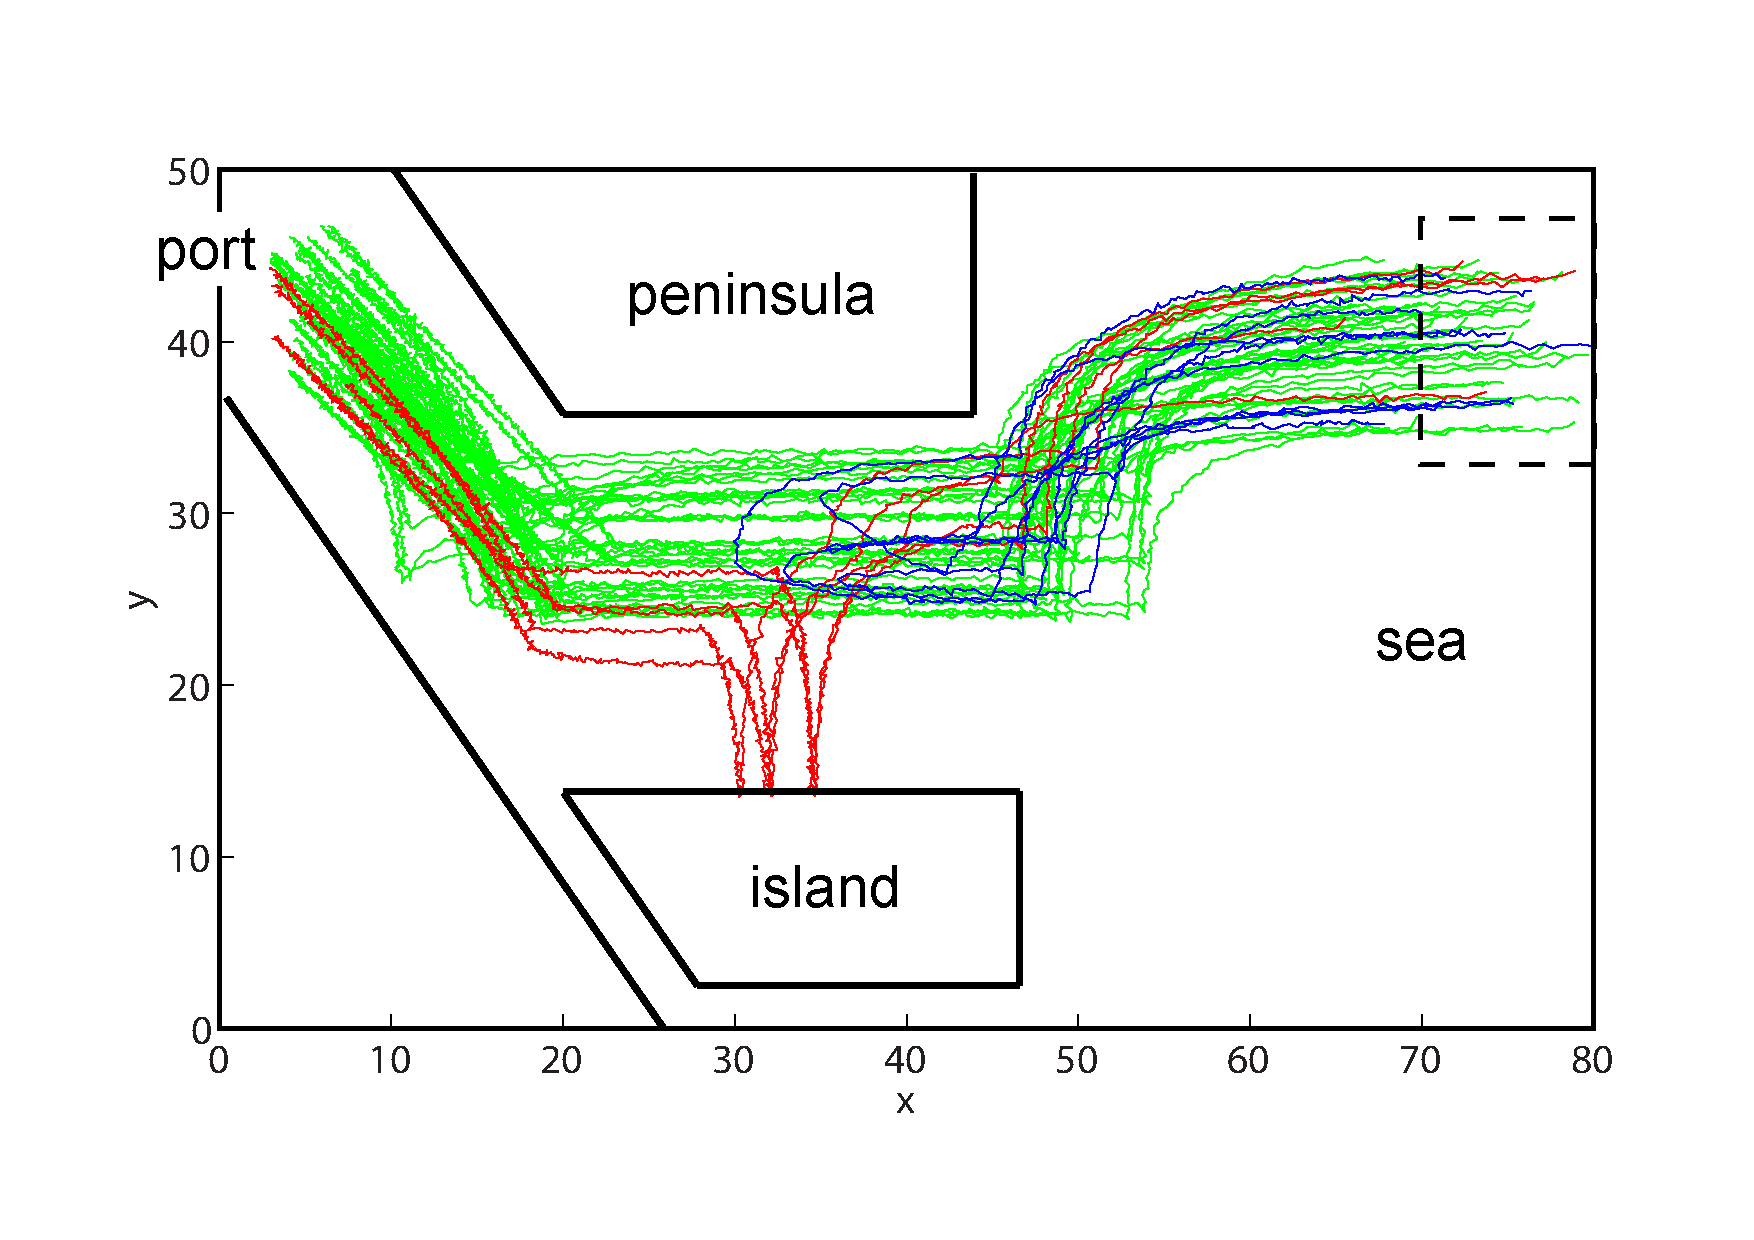
\includegraphics[width=1.0\columnwidth]{naval_sample}
  \caption{Naval surveillance dataset - The vessels behaving normally are shown in green. The red and blue traces represent two types of anomalous paths (human trafficking and terrorism, respectively).}\label{fig:naval_sample}
\end{figure}


\subsection{Fuel control system}
We investigate a fuel control system for a gasoline engine. A model for this system is provided as built-in example in Simulink \cite{SimulinkGuideFTFCS} and we modified it for our purposes.
This model was initially used for Bayesian statistical model checking \cite{zuliani_bayesian_2013} and has been recently proposed as benchmark for the Hybrid Systems community \cite{hoxha_benchmarks_2014}.
We selected this model because it includes all the complexities of real world industrial models, but is still quick to simulate, i.e., it is easy to obtain a large number of trajectories.

\begin{figure}
  \centering
  \includegraphics[width=1.0\columnwidth]{fcs_overview}
  \caption{Fuel Control - Overview of the model (modified from \cite{SimulinkGuideFTFCS})}\label{fig:fcs_overview}
\end{figure}
The key quantity in the model is the \emph{air-to-fuel ratio}, that is, the ratio between the mass of air and the mass of fuel in the combustion process. The goal of the control system is to keep it close to the ``ideal'' stoichiometric value for the combustion process.
For this system, the target air-fuel ratio is $14.6$, as it provides a good compromise between power, fuel economy, and emissions. An overview of the Simulink diagram is shown in Figure \ref{fig:fcs_overview}.
There is one main output, the air-to-fuel ratio, one control variable, the fuel rate, and two inputs, the engine speed and the throttle command.
The system estimates the correct fuel rate to achieve the target stoichiometric ratio by taking into account four sensor readings.
Two are related directly to the inputs, the engine speed and the throttle angle. The remaining two sensors provide crucial feedback information: the EGO sensor reports the amount of residual oxygen present in the exhaust gas, and the MAP sensor reports the (intake) manifold absolute pressure.
The EGO value is related to the air-to-fuel ratio, whereas the MAP value is related to the air mass rate.
The diagram in Figure \ref{fig:fcs_overview} is made of several subsystems with different kinds of blocks within, both continuous and discrete, among which there are look-up tables and a Stateflow chart.
Due to these characteristics, this model can exhibit a rich and diverse number of output trajectories, thus making it an interesting candidate for our investigation.

%\subsubsection{Modifications and fault injections}\label{sec:mod_faults}
\begin{figure}
  \centering
  \includegraphics[width=1.0\columnwidth]{fcs_sensorfaults}
  \caption{Fuel Control - Sensor Faults Injection}\label{fig:fcs_sensorfaults}
\end{figure}

The base model, that is, the one included in Simulink, includes a very basic fault detection scheme and fault injection mechanism.
The fault detection scheme is a simple threshold crossing test (within the Stateflow chart), and is only able to detect single off range values. For avoiding the overlap of two anomaly detection schemes, the built-in one has been removed.
In the base model, the faults are injected by simply reporting an incorrect and fixed value for a sensor's reading. Moreover, these faults are always present from the beginning of the simulation. We substituted this simple fault injection mechanism with a more sophisticated unit.
The new subsystem, shown in Figure \ref{fig:fcs_sensorfaults}, is capable of inducing faults in both the EGO and MAP sensors with a \emph{random} arrival time and with a \emph{random} value.
Specifically, the faults can manifest at anytime during the execution (uniformly at random) and the readings of the sensors affected 
%by a fault 
are offset by a value that \emph{varies} at every execution.
Finally, independent Gaussian noise signals, with zero mean and variance $\sigma^2 = 0.01$, have been added at the output of the sensors. 
% and for the initial conditions of the system.

%\subsubsection{Dataset generation}\label{sec:datasets}
For the fuel control system, $1200$ total simulations were performed.
In all cases, the throttle command provides a periodic triangular input, and the engine speed is kept constant at $300$ rad/sec ($2865$ RPM). The simulation time is $60$ seconds. In details, we obtained:
\begin{itemize}
\item 600 traces where the system was working normally;
\item 200 traces with a fault in the EGO sensor;
\item 200 traces with a fault in the MAP sensor;
\item 200 traces with faults in both sensors.
\end{itemize}
For every trace we collected the values of the air-to-fuel ratio ($x_1$), the fuel rate ($x_2$), and the EGO and MAP sensors' readings  ($x_3$ and $x_4$).
The average simulation time for obtaining a single trace was roughly $1$ second. 
\section{Results}\label{sec:results}
%\subsection{Joe's results}

\subsubsection{Maritime Surveillance}
%\subsubsection{Results}
We randomly split the dataset in half, and used 1000 traces for training and 1000 traces for testing.
\[
\big( (G_{[94.6,300)} x_{2}<35.3) \wedge (G_{[0,300)} x_{2}>23) \wedge (G_{[298,300)} x_{1}<25.9) \big)  \vee \big( (F_{[94.6,300)} x_{2}>35.3) \wedge (G_{[182,300)} x_{1}<19.6) \wedge (G_{[0,51.6)} x_{1}>42.6) \big)
\]
mcr=0.0040;
time=23min;


%The formula inferred in \cite{kong_temporal_2015} had a misclassification rate 8.85\% on the training data with a computation time of 648 s (approx. 11 minutes).


\subsubsection{Fuel control system}
\[
\big( (G_{[0,59.7)} x_{2}>-0.563) \wedge (G_{[0,59.7)} x_{2}<1.91) \wedge (G_{[0,59.7)} x_{1}>-0.819) \wedge (G_{[23.7,59.7)} x_{1}<1.78) \big)
\]
MCR=0.0541
mcr=0.0040;
time=17min;


\subsection{Fran's results}
\begin{algorithm}
\caption{Tree to formula -- $Tree2STL(\cdot)$}
\label{alg:tree2formula}
\DontPrintSemicolon
\KwIn{$node$ -- Starting node of a tree}
\KwOut{Formula}
\BlankLine

\uIf{$node$ is $leaf$}{
    \Return{$\True$}
}

$\phi \asgn$ formula associated with $node$

\uIf{$node.right$ is $leaf$}{
    \Return{$\phi \andltl Tree2STL(node.left)$}
}\Else{
    \Return{$(\phi \andltl Tree2STL(node.left)) \orltl (\notltl \phi \andltl Tree2STL(node.right))$}
}
\end{algorithm}



%\input{text/conclusion}

%
% The following two commands are all you need in the
% initial runs of your .tex file to
% produce the bibliography for the citations in your paper.
\bibliographystyle{abbrv}
\bibliography{references}  % sigproc.bib is the name of the Bibliography in this case
% You must have a proper ".bib" file
%  and remember to run:
% latex bibtex latex latex
% to resolve all references
%
% ACM needs 'a single self-contained file'!
%
%APPENDICES are optional
%\balancecolumns
\appendix
%Appendix A
\input{text/appendices}
\clearpage
\section{Look-up table computation of robustness}
\begin{proposition}
\label{th:primitives-props}
Let $s$ be an $n$-dimensional signal. The following hold:
\begin{enumerate}
    \item the sets of primitives $\CA{P}_1$ and $\CA{P}_2$ are
    closed under negation, i.e. $\phi \in \CA{P} \Implies \notltl\phi \in \CA{P}$,
    where $\CA{P}$ is $\CA{P}_1$ or $\CA{P}_2$;
    \item robustness  of 1$^{st}$ order primitives:
    \begin{align}
    	r(s, \Event_{[\tau_1, \tau_2)} (s_i \leq \mu)) &= \inf_{t \in [\tau_1, \tau_2)} \{ s_i(t) \} - \mu \\
    	r(s, \Always_{[\tau_1, \tau_2)} (s_i \leq \mu)) &= -\inf_{t \in [\tau_1, \tau_2)} \{ -s_i(t) \} - \mu
    \end{align}
    \item robustness  of 2$^{nd}$ order primitives:
    \begin{align}
    	r(s, \varphi_{\Event\Always}) &= \inf_{t_1 \in [\tau_1, \tau_2)} \big\{  \sup_{t_2 \in [0, \tau_3)} \{ s_i(t) \} \big\} - \mu \\
    	r(s, \varphi_{\Always\Event}) &= -\inf_{t_1 \in [\tau_1, \tau_2)} \big\{  \sup_{t_2 \in [0, \tau_3)} \{ -s_i(t) \} \big\} - \mu
    \end{align}
    where $\varphi_{\Event\Always} = \Event_{[\tau_1, \tau_2)} \Always_{[0, \tau_3)} (s_i \leq \mu)$
    and \quad $\varphi_{\Always\Event} = \Always_{[\tau_1, \tau_2)} \Event_{[0, \tau_3)} (s_i \leq \mu)$.
\end{enumerate}
\end{proposition}
\begin{proof}
The proof follows immediately from the definitions of the eventually and always operators and of the robustness.
\end{proof}




{\color{orange}
TODO: informal description. If we include this
in the paper, we need to massage it.
NOTE: I think we can remove the algorithms
from this version of the paper
(comment to latex code please) and just
briefly explain how it works.

If we consider piecewise constant (or linear)
signals obtained by uniform sampling, i.e.
at constant rate, then we can speed-up
robustness computation by pre-computing
lookup tables for each signal before the
inference algorithm is executed.
For each signal $s$, we compute the robustness
degree of $s$ and $-s$ for every possible
valuation of the 2 and 3 time parameters
of primitives in $\CA{P}_1$ and $\CA{P}_2$,
respectively. The space parameter $\mu$ is set
to 0.
By Prop.~\ref{th:primitives-props}, the computation
of robustness reduces to a lookup in a table,
the subtraction of $\mu$ and a possible change of sign.

For the set of primitives $\CA{P}_2$, the lookup
tables can efficiently be computed as
shown in Alg.~\ref{alg:lkt-1d}, Alg.~\ref{alg:lkt-nd}
and Alg.~\ref{alg:lkt-prim}. The robustness is
computed usinf the lookup table in
Alg.~\ref{alg:robustness-lookup}.

The size of the lookup tables for all signals $S$ is
$2\times \card{S} \times n \times T^3$, where $n$ is the
dimension of the signals, $T$ is the number
of samples per signal, and 2 in the expression
indicates that we compute two lookup tables per
signal, one for each type of primitive.

Another approach is to save the entries of the
lookup table as these are computed during the
optimization procedure. In this way, later
operations will not have to recompute these.
This approach is in line with lazy-computation
heuristics.
}

\begin{algorithm}
\caption{Lookup table for 1d signal -- $lkt\_1d(\cdot)$}
\label{alg:lkt-1d}
\DontPrintSemicolon
\KwIn{$s$ -- signal}
\KwOut{Lookup table}
\BlankLine

$T \asgn length(s)$ \tcp*[f]{number of samples per signal}\;
$lk1 \asgn fill((T, T), \infty)$\;
$lk1[0, 0:T] \asgn s$\;
\For{$i = 1 \text{ to } T$}{
  $n \asgn T - i$\;
  $lk1[i, 0:n] \asgn pmin(lk1[i-1, 0:n], lk1[i-1, 1:n+1])$\;
}
$lk \asgn fill((T, T, T), -\infty)$\;
\For{$\tau_3 = 0 \text{ to } T$}{
  $n \asgn T - \tau_3$\;
  $lk[0:n, 0, \tau_3] \asgn lk1[\tau_3, 0:n]$\;
  \For{$j = 1\text{ to } n$}{
    $m \asgn n - j$\;
    $lk[0:m, j, \tau_3] \asgn pmax(lk[0:m, j-1, \tau_3],$\;
    \qquad\qquad\qquad\qquad\qquad\  $lk[1:m+1, j-1, \tau_3])$\;
  }
}
\Return{$lk$}
\end{algorithm}

\begin{algorithm}
\caption{Lookup table for n-dimensional signal -- $lkt\_nd(\cdot)$}
\label{alg:lkt-nd}
\DontPrintSemicolon
\KwIn{$s$ -- signal}
\KwOut{Lookup table}
\BlankLine

$lk \asgn fill((n, T, T, T), -\infty)$\;
\For{$i = 0 \text{ to } n$}{
  $lk[i, 0:T, 0:T, 0:T] \asgn lkt\_1d(s_i)$
}
\Return{$lk$}
\end{algorithm}

\begin{algorithm}
\caption{Lookup tables -- $lkt\_prim(\cdot)$}
\label{alg:lkt-prim}
\DontPrintSemicolon
\KwIn{$S$ -- set of signals}
\KwOut{Lookup table}
\BlankLine

$lk\_max\_min \asgn fill((\card{S}, n, T, T, T), 0)$\;
\For{$s \in S$}{
  $lk\_max\_min[s, 0:n, 0:T, 0:T, 0:T] \asgn lookup\_nd(s)$
}
$lk\_min\_max \asgn fill((\card{S}, n, T, T, T), 0)$\;
\For{$s \in S$}{
  $lk\_min\_max[s, 0:n, 0:T, 0:T, 0:T] \asgn -lookup\_nd(-s)$
}
\Return{$(lk\_max\_min, lk\_min\_max)$}
\end{algorithm}

\begin{algorithm}
\caption{Robustness -- $robustness(\cdot)$}
\label{alg:robustness-lookup}
\DontPrintSemicolon
\KwIn{$s$ -- signal}
\KwIn{$\phi$ -- primitive in $\CA{P}_2$}
\KwIn{$(lk\_max\_min, lk\_min\_max)$ -- lookup tables}
\KwOut{robustness}
\BlankLine

$i_1, i_2, i_3 \asgn \lfloor\tau_1\rfloor, \lceil\tau_2 - \tau_1\rceil, \lceil \tau_3\rceil$

\uIf{$F_{[\tau_1, \tau_2]} G_{[0, \tau_3]} (s^j \leq \mu)$}{
  \Return{$lk\_max\_min[s, j, i_1, i_2, i_3] - \mu$}
}
\uElseIf{$G_{[\tau_1, \tau_2]} F_{[0, \tau_3]} (s^j > \mu)$}{
  \Return{$\mu - lk\_max\_min[s, j, i_1, i_2, i_3]$}
}
\uElseIf{$G_{[\tau_1, \tau_2]} F_{[0, \tau_3]} (s^j \leq \mu)$}{
  \Return{$lk\_min\_max[s, j, i_1, i_2, i_3] - \mu$}
}
\ElseIf{$F_{[\tau_1, \tau_2]} G_{[0, \tau_3]} (s^j > \mu)$}{
  \Return{$\mu - lk\_min\_max[s, j, i_1, i_2, i_3]$}
}

%def robustness_lookup(t0, t1, t3, mu, sindex, pred_less, ev_al, traces):
%    '''Robustness lookup for primitives
%    F_{[t_0, t_1]} (G_{[0, t_3]} (s_{sindex} \leq mu)), if ev_al is true,
%    G_{[t_0, t_1]} (F_{[0, t_3]} (s_{sindex} \leq mu)), otherwise.
%    If pred_less is False then the predicate is assumed to be negated, i.e. gt.
%    '''
%    t0, t1, t3 = np.floor(t0), np.ceil(t1), np.ceil(t3)
%    sgn = 1 if pred_less else -1
%    if ev_al:
%        return sgn*(traces.traces_lkt_max_min[:, sindex, t0, t1-t0, t3] - mu)
%    return sgn*(traces.traces_lkt_min_max[:, sindex, t0, t1-t0, t3] - mu)
\end{algorithm}

%\subsection{Figures}
%
%\begin{figure}
%\centering
%\epsfig{file=fly.eps}
%\caption{A sample black and white graphic (.eps format).}
%\end{figure}
%
%\begin{figure}
%\centering
%\epsfig{file=fly.eps, height=1in, width=1in}
%\caption{A sample black and white graphic (.eps format)
%that has been resized with the \texttt{epsfig} command.}
%\end{figure}
%
%\begin{figure}
%\centering
%\psfig{file=rosette.ps, height=1in, width=1in,}
%\caption{A sample black and white graphic (.ps format) that has
%been resized with the \texttt{psfig} command.}
%\end{figure}
%
%\begin{figure*}
%\centering
%\epsfig{file=flies.eps}
%\caption{A sample black and white graphic (.eps format)
%that needs to span two columns of text.}
%\end{figure*}



\balancecolumns
% That's all folks!
\end{document} 